\epigraph{Give me a place to stand and I will move the earth.}{Archimedes.}

In this chapter, I provide background knowledge on three main topics, namely
language model (LM), recurrent neural network (RNN), and neural machine
translation (NMT).
Language modeling is an important concept in natural language processing to
allow one to do {\it word prediction}, i.e., guessing which word will come next
given a preceding context. As we shall see later, there is an interesting fact
that for neural machine
translation, it all started from language modeling. Before I get into NMT, 
we will go through the basics of recurrent neural network, the heart of
sequence-based NMT, to
explain how RNNs can naturally and effectively model {\it variable-length} inputs, or
sentences in the context of the translation task. 
I cover in depth one particular type of RNN, the {\it Long Short-term Memory}
(LSTM), that makes training RNNs easier. Interested readers can find all the
details of how to implement LSTM ``by hand'' with detailed formulas on gradient
computation as compared to the automatic differentiation feature given by nowadays deep
learning frameworks. The understanding of language modeling will allow us
to extend RNNs into recurrent neural language models which enable {\it language
generation}, a key step in NMT.
Lastly, with RNN as a basic building block, I describe key elements of an NMT
system as well as tips and tricks for better training and testing NMT.

\section{Language Model}
As I have discussed in \secref{sec:mt}, language modeling plays an indispensable
role in MT to ensure that systems produce fluent translations.
Specifically, the job of an LM is to specify a probability distribution over
sequences of symbols (often, words) so that one can judge if a sequence of
words is more likely or ``fluent'' than another. To accomplish that, an LM
decomposes the probability of a word sequence $y = y_1, \ldots, y_m$ as:
\begin{align}
p(y) = \prod_{i=1}^m p(y_i | y_{<i}) %\yrange{1}{i-1})
\end{align}
In the above formula, each of the
individual terms $p(y_i | y_{<i})$ is the conditional probability of the current
word $y_i$ given previous words $y_{<i}$, also referred to as the {\it
context} or the {\it history}. 
To model these conditional probabilities, traditional \ngram{}
 LMs have to resort to the %as well as feedforward-based neural
Markovian assumption to consider only a fixed context window of $n\!-\!1$ words,
effectively modeling $p(y_i | y_{i-n+1}, \ldots, y_{i-1})$. 
In fact, \ngram{} LMs have to explicitly store and handle 
all possible \ngram{}s occurred in a training corpus, the number of which
quickly becomes enormous. As a result, 
despite much research in this area 
\cite{rosenfeld2000,srilm,teh2006,irstlm,kenlm}, inter alia, %,pauls2011,heafield13
\ngram{} LMs can only handle short contexts of about 4 to 6 words,  
and does not generalize well to unseen \ngram{}s. 

Neural language models (NLMs), first proposed by \newcite{Bengio2003} and enhanced by
others such as \newcite{Morin2005,MnihHinton2009,MnihTeh2012}, have addressed the
aforementioned concerns using two ideas: 
(a) {\it dense distributed representations} for words which encourage sharing
of statistical weights between similar words; and (b) {\it feed-forward neural
networks} to allow for better composition of unseen word sequences at test time
without having to explicitly store all enumerations of \ngram{}s. 
These features function as a way to combat the ``curse'' of dimensionality
in language modeling. As a result, NLMs are compact and can extend to longer
context.

As a natural development, subsequent MT systems
\cite{schwenk07,vaswani13decode,luong15nlm}, inter alia, started adopting NLMs
alongside with traditional \ngram{} LMs and generally obtain sizable
improvements in terms of translation quality.
To make NLMs even more powerful, recent work
\cite{Schwenk12continuous,Son:2012:CST,Auli13,devlin14}
proposes to condition on source words as well as the target context to lower
uncertainty in predicting next words (see Figure~\ref{f:nnjm}).\footnote{In
\cite{devlin14}, the authors constructed a model that conditions on 3
target words and 11 source words, effectively building a $15$-gram LM.}
These hybrid MT systems with \nlm{} components, while better than statistical MT
systems, still translate locally and fail to capture long-range dependencies.
For example, in Figure~\ref{f:nnjm}, the
source-conditioned \nlm{} does not see the word \word{stroll}, or any other words
outside of its fixed context windows, which can be useful in deciding that the
next word should be \word{bank} as in \word{river bank} rather \word{financial
bank}. 
\begin{figure}[tbh!]
\centering
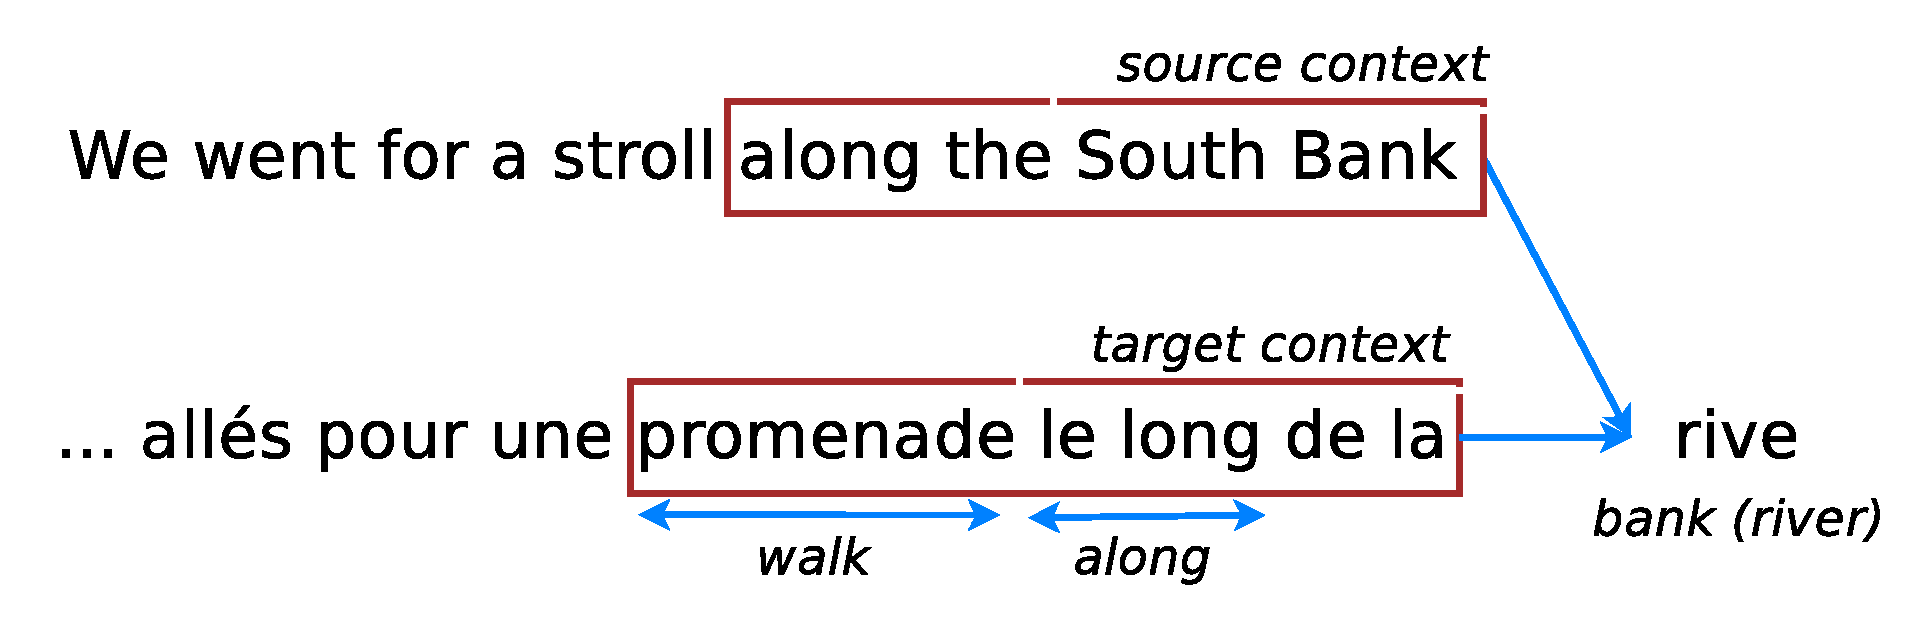
\includegraphics[width=0.7\textwidth, clip=true, trim= 0 0 0 0]{img/nnjm.eps} % , angle=-90
\caption[Source-conditioned \nlmtext{}]{{\bf Source-conditioned \nlmtext{}}
(\nlms{}) -- example of a source-conditioned
\nlm{} proposed by \newcite{devlin14}. To evaluate how likely a next word
\word{rive} is, the model not only relies on previous target words (context)
\word{promenade le long de la} as in
traditional \nlms{} \cite{Bengio2003}, but also utilizes source context \word{along the
South Bank} to lower uncertainty in its prediction.
} 
\label{f:nnjm}
\end{figure}

More problematically, the entire MT pipeline is already complex with
different components needing to be tuned separately such as translation models,
language models, and reordering models. Now, it becomes even worse as
different neural components are incorporated in to the translation framework.
This inspires the birth of neural machine
translation with a goal of redesigning the entire MT pipeline completely. To start, we will
first learn about recurrent neural network, a
building block for NMT as well as a key component to address the local
translation problem in statistical MT systems.

\section{Recurrent Neural Network}
\label{sec:rnn}
\edit{
%Recurrent Neural Network (RNNs) \cite{elman90} are models that help understand
%the temporal aspect as well as build up representations for sequential data
%using a dynamic memory structure. At the surface form
Recurrent neural network (RNN) \cite{elman90} is a powerful and expressive
architecture that can handle sequential data and has been successfully applied to 
language modeling tasks \cite{MikolovKBCK10,MikolovKBCK11,mikolovLM}.
}
Formally, an RNN takes as input a sequence of vectors $\x{1},
\x{2}, \ldots, \x{n}$ and processes them one by one. For each
new input $\x{i}$, an RNN updates its memory to produce a hidden state
$\hid{i}$ which one can think of as a representation for the partial sequence
$\x{\overline{1,i}}$. %$\x{1},\ldots, \x{i}$. 
The key secret sauce is in the
recurrence formula of an RNN that defines how its hidden state is updated. At
its simplest form, a ``vanilla'' RNN defines its recurrence function as:
\begin{align}
\hid{t} &= f\paren{\x{t}, \hid{t-1}} \label{e:abstract_rnn}
\end{align}
In the above formula, $f$ is an abstract function that computes a new hidden state given the current input $\x{t}$ and the
previous hidden state $\hid{t-1}$. The starting state $\hid{0}$ is often set to
$\bm{0}$ though it can take any value as we will see later in the context
of NMT decoders. A popular choice of $f$ is provided below with $\sigma$ being a
non-linear function such as $\sigmoid$ or $\tanh$.\footnote{There could also be
an optional bias term in \eq{e:vanilla_rnn}.}
\begin{align}
%\z{t} &= \W{xh}\x{t} + \W{hh}\hid{t-1} \label{e:vanilla_rnn} \\
\hid{t} &= \sigma(\W{xh}\x{t} + \W{hh}\hid{t-1} \label{e:vanilla_rnn}) %\z{t})
\end{align}

At each timestep $t$, an RNN can (optionally) emit an output symbol
$y_t$ which can either be discrete or real-valued. For the discrete scenario,
which is often the case for linguistic applications, a probability distribution $\bm{p}$ over a 
set of output classes $Y$ is derived as:\footnote{For the real-valued case, I refer readers to mixture density
models \cite{bishop94} which have been applied to RNN training, e.g., for
hand-writing synthesis \cite{graves13c}.}
\begin{align}
\s{t} &= \W{hy}\hid{t} \label{e:score} \\
\prob{t} &= \softmax(\s{t}) \label{e:prob}
\end{align}
Here, I introduce a new set of weights $\W{hy} \inR{|Y| \times d}$, with $d$ being the dimension of the RNN hidden
state, to compute a score vector $\s{t}$, or {\it logits}, over
different individual classes. Often, with a large output set $Y$, the
matrix-vector multiplication in \eq{e:score} is a major computational
bottleneck in RNNs, which results in several challenges for neural language modeling
and machine translation that I will address in later chapters. 
The $\softmax$ function transforms the score
vector $\s{t}$ into a probability vector $\prob{t}$, which is defined for each specific
element $y \in Y$ as below.
For convenience, we overload our notations to use $\prob{t}(y)$ and $\s{t}(y)$ to refer to entries in
the vectors $\prob{t}$ and $\s{t}$ that correspond to $y$.
\begin{align}
\prob{t}(y) = \frac{e^{\s{t}(y)}}{\sum_{y' \in Y} e^{\s{t}(y')}}
\label{e:softmax}
\end{align}

With the above formulas, I have completely defined the RNN weight set $\thetav$
%=\!\{\W{xh}, \W{hh}, \W{hy}\}$, 
which consists of {\it input} connections $\W{xh}$, {\it
recurrent} connections $\W{hh}$, and {\it output}
connections $\W{hy}$. These weights are shared across
timesteps as illustrated in Figure~\ref{f:rnn}. %, which enables RNNs to handle arbitrarily long sequences.
\edit{This is, in fact, the beauty of RNNs as they can
capture the dynamics of arbitrarily long sequences without having to increase
their modeling capacity. In contrast, feedforward networks can only model
relationship over fixed-length segments. 

\begin{figure}[tbh!]
\centering
%\psgrid
\rput(8.2,3.5){{\color{lightred} $\W{hy}$}}
\rput(7.7,2.5){{\color{lightblue} $\W{hh}$}}
\rput(8.2,0.9){{\color{lightgreen} $\W{xh}$}}
\rput(8.9,0.3){{\color{lightgreen} $\x{n}$}}
\rput(6.9,0.3){{\color{lightgreen} $\ldots$}}
\rput(5.1,0.3){{\color{lightgreen} $\x{2}$}}
\rput(3.3,0.3){{\color{lightgreen} $\x{1}$}}
\rput(8.9,4.2){{\color{lightred} $\y{n}$}}
\rput(6.9,4.2){{\color{lightred} $\ldots$}}
\rput(5.1,4.2){{\color{lightred} $\y{2}$}}
\rput(3.3,4.2){{\color{lightred} $\y{1}$}}
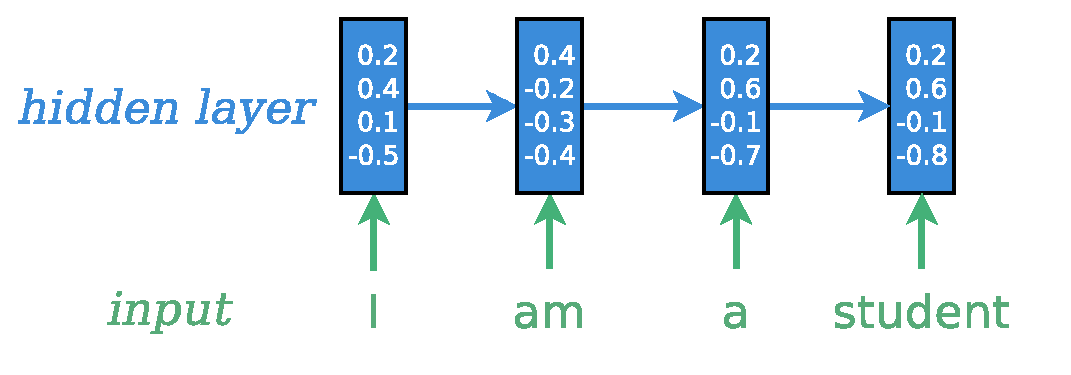
\includegraphics[width=0.6\textwidth, clip=true, trim= 0 0 0 0]{img/rnn.eps} % , angle=-90
\caption[Recurrent neural networks]{{\bf Recurrent neural networks} -- example of a recurrent
neural network that processes a input sequence $\x{1}, \x{2}, \ldots, \x{n}$ to
build up hidden representations as each input is consumed and produces an output
sequence $\y{1}, \y{2}, \ldots, \y{n}$. The input $\MB{W_{xh}}$, recurrent
$\MB{W_{hh}}$, and output $\MB{W_{hy}}$  weights are shared across timesteps.
} 
\label{f:rnn}
\end{figure}
}
Throughout this thesis, RNNs will be discussed from a language
learning perspective. For more details on general RNNs, I refer readers to the
following resources \cite{sutskever12,mikolov12,karpathy15rnn}.

\paragraph{Recurrent Language Models}
%\label{subsec:rlm}
\edit{
As a special case of RNN, recurrent language model assumes that the input and output
sequences consist of discrete symbols, often words in a language.
Additionally, the input sequence is prepended with a special starting symbol
\sos{}, e.g., $x=\{$ \sos, ``I'', ``am'', ``a'', ``student''$\}$.
Since the goal of a language model is to predict the next word, the output
sequence is a shift-by-1 version of the input and ends
with a special symbol \eos{} that marks the boundary, e.g., $y=\{$ ``I'', ``am'', ``a'',
``student'', \eos$\}$. As I illustrate in \figref{f:rlm}, the word emitted at
one timestep is used as an input to the next timestep.
}

\begin{figure}[tbh!]
\centering
%\psgrid
\rput(9,4.6){{\color{lightred} $\W{hy}$}}
\rput(8.7,3.9){{\color{lightblue} $\W{hh}$}}
\rput(9,2.5){{\color{lightgreen} $\W{xh}$}}
\rput(1.4,1.3){{\color{lightpurple} $\W{e}$}}
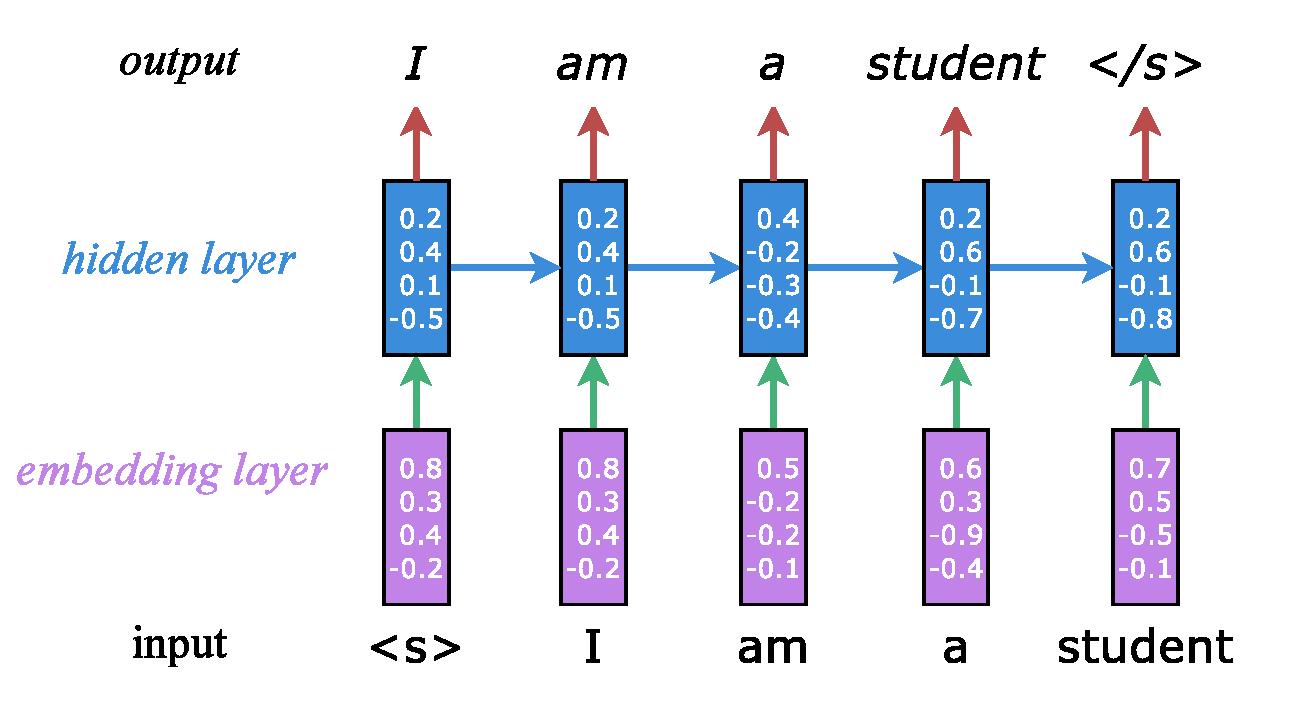
\includegraphics[width=0.7\textwidth, clip=true, trim= 0 0 0 0]{img/rnnlm.eps} % , angle=-90
\caption[Recurrent language models]{{\bf Recurrent language models} -- example of a recurrent
language model that processes a sentence \word{I am a student} and predicts next
words as it goes. \edit{Beside the shared recurrent $\W{hh}$ and feed-forward $\W{xh}$
weights, there is an additional shared embedding weight matrix $\W{e}$ that needs to be
learned as well.}
} 
\label{f:rlm}
\end{figure}

To apply RNNs to sentences in languages, or generally sequences of discrete symbols, one can
consider one-hot representations for words, i.e., $\x{i} \inR{|V|}$, with $V$ being the
vocabulary considered. However, for a large
vocabulary $V$, such a representation choice is problematic as it results in
a large weight matrix $\W{xh}$ and there is no notion of similarity between
words. In practice, low-dimensional dense representations for words, or {\it
embeddings}, are often used to address these problems. Specifically, an
embedding matrix
$\W{e} \inR{d_e \times |V|}$ is looked up for each word $x_i$ to retrieve a
representation $\x{i} \inR{d_e}$. As a result, a vanilla recurrent language model
will generally have $\theta = \{\W{xh}, \W{hh}, \W{hy}, \W{e}\}$ as its
weights. % as illustrated in Figure~\ref{f:rlm}. 

\subsection{Training \& Backpropagation}
Given a training dataset of $N$ discrete output sequences $\ytop{1}, \ldots,
\ytop{N}$ with lengths $m_1, \ldots, m_N$ accordingly. The learning objective is
to minimize the negative log-likelihood, or the {\it cross-entropy} loss, of these training examples:
\begin{align}
J(\thetav) &= \sum_{i=1}^{N} -\log p\paren{\ytop{i}} \\ 
&= \sum_{i=1}^{N} \sum_{t=1}^{m_i} -\log p\paren{\ytop{i}_t |
\ytop{i}_{<t}}
\label{e:objective}
\end{align}

RNN learning is often done using mini-batch stochastic gradient descent (SGD) algorithms in
which a small set of training examples, a {\it mini-batch}, is used to compute
the gradients and update weights one at a time. Using mini-batches has
several advantages: (a) the gradients are more reliable and consistent than the
``online'' setting which updates per example, (b) less computation is required to
update the weights unlike the case of full-batch learning which has to process
all examples before updating, and (c) with multiple examples in a mini-batch,
one can turn matrix-vector multiplications such
as those in \eq{e:vanilla_rnn} and \eq{e:score} into matrix-matrix multiplications which can be
deployed efficiently on GPUs. The simplest weight update formula with $\eta$ as
a learning rate is given below:
\begin{align}
\thetav \longleftarrow \thetav - \eta \grad{J(\thetav)} %\fracder{J(\thetav)}{\thetav}
\end{align}
\edit{Here, $\grad{J(\thetav)}$ is the gradient of the loss that we are
minimizing with respect to the model weights. Intuitively, what the formula does is to update the weights along the
opposite direction of the gradient to minimize the loss objective. The learning
rate $\eta$, sometimes referred as a {\it step size}, is a hyperparameter which
controls how much we update the weights along the optimization direction.}

\paragraph{Mathematical Helpers}
%\label{ss:misc}
\edit{To simplify the maths for our backpropagation derivations in the next
section, I present here a few simple remarks and lemmas on vector calculus and gradient
computation.}

\begin{remark}
\label{r:diag_mul}
Let $\bm{u}$, $\bm{v}$ be any vectors and $\edot$ be element-wise vector multiplication, we have:
\begin{align}
\diag (\bm{u}) \cdot \bm{v} = \bm{u} \edot \bm{v}
\end{align}
\edit{Here $\diag (\bm{u})$ refers to a diagonal matrix with its diagonal
elements being $\bm{u}$.}
\end{remark}

\begin{lemma}
\label{l:chain_rule}
Let $l$ be a loss value for which we
already know how to compute its gradient $\der{v}$ with respect to a vector $\bm{v}$. Given that
$\bm{v} = f(\bm{Wh})$, the gradients $\der{h}, \der{W}$ of the loss $l$ with respect to the vector
$\bm{h}$ and the matrix $\bm{W}$ can be derived as follows:
\begin{align}
\der{h} = \tp{\bm{W}} \cdot \paren{f'(\bm{Wh}) \edot \der{v}}
\\
\der{W} = \paren{f'(\bm{Wh}) \edot \der{v}} \cdot \tp{\bm{h}} 
\end{align}
\end{lemma}

\begin{proof}
Let $\bm{z} = \bm{Wh}$, we have the following derivations: %applying chain rules in vector calculus, 
\begin{align*}
\der{h} &= \fracder{\bm{z}}{\bm{h}} \cdot \fracder{\bm{v}}{\bm{z}}
\cdot \der{v} && \text{[Vector calculus chain rules]}\\
&= \fracder{\bm{Wh}}{\bm{h}} \cdot \fracder{f(\bm{z})}{\bm{z}}
\cdot \der{v} \\
&=\tp{\bm{W}} \cdot \diag \paren{f'(\bm{z})} \cdot \der{v} \\
&=\tp{\bm{W}} \cdot \paren{f'(\bm{Wh}) \edot \der{v}} &&
\text{[\remarkref{r:diag_mul}]}
\end{align*}

Let $\tp{\bm{w}_i}$ be the $i^{\text{th}}$ row vector of matrix $\bm{W}$ and
$v_i, z_i$ be the $i^{\text{th}}$ elements of vectors $\bm{v}, \bm{z}$. Also
denoting $\der{w}_i, dv_i$ to be the gradients of $l$ with respect to $\bm{w}_i,
v_i$, we have:
\begin{align*}
d\bm{w}_i &= \fracder{z_i}{\bm{w}_i} \cdot \fracder{v_i}{z_i}
\cdot dv_i && \text{[Vector calculus chain rules]}\\
&= \fracder{\tp{\bm{w}_i}\bm{h}}{\bm{w}_i} \cdot f'(z_i) \cdot dv_i \\
&= \bm{h} \cdot f'(z_i) \cdot dv_i \\ 
d\tp{\bm{w}_i} &= \paren{f'(z_i) \cdot dv_i} \cdot
\tp{\bm{h}} && \text{[Transposing]} \\
\der{W} &= \paren{f'(\bm{Wh}) \edot \der{v}} \cdot \tp{\bm{h}}
&& \text{[Concatenating row derivatives]}
\end{align*}
\end{proof}

\begin{corollary}
\label{c:chain_rule}
As a special case of \lemmaref{l:chain_rule}, when $f$ is an identity function,
i.e., $\bm{v} = \bm{Wh}$, we have:
\begin{align}
\der{h} = \tp{\bm{W}} \cdot \der{v}
\\
\der{W} = \der{v} \cdot \tp{\bm{h}} 
\end{align}
\end{corollary}

\begin{remark}
\label{r:edot_der}
Let $\bm{u}$, $\bm{v}, \bm{s}$ be any vectors such that  $\bm{s} = \bm{u} \edot
f(\bm{v})$. Also, let $d\bm{u}$, $d\bm{v}, d\bm{s}$ be the gradients of a loss $l$ with
respect to the corresponding vectors. We have:
\begin{align}
d\bm{u} = f(\bm{v}) \edot d\bm{s} \\
d\bm{v} = f'(\bm{v}) \edot \bm{u} \edot d\bm{s} 
\end{align}
\end{remark}

\begin{remark}
\label{r:edot_der2}
As a special case of \remarkref{r:edot_der} when $f$ is an identity function,
i.e.,  $\bm{s} = \bm{u} \edot \bm{v}$. We have:
\begin{align}
d\bm{u} = \bm{v} \edot d\bm{s} \\
d\bm{v} = \bm{u} \edot d\bm{s} 
\end{align}
\end{remark}



\paragraph{Single-Time Backpropagation} To compute the gradients for the loss $J(\thetav)$,
we first need to be able to derive the gradients of the per-timestep loss $l_t
=-\log \prob{t}(y_t)$ with respect to both the RNN weights
$\{\W{xh}, \W{hh}, \W{hy}\}$ and the inputs $\{\x{t}, \hid{t-1}\}$. It is worth
noting that
$\x{t}$ is a column vector in the embedding matrix $\W{e}$. We denote
these gradients as $\{d\W{xh}, d\W{hh}, d\W{hy}, d\x{t}, d\hid{t-1}\}$
respectively and define intermediate gradients $d\s{t}, d\hid{t}$ similarly
with $\s{t}$ and $\hid{t}$ being used in \eq{e:score} and \eq{e:prob}. 
Starting with the loss $l_t$, we employ backpropagation through structures
\cite{goller96} to derive each gradient one by one in the following
order: $l_t \rightarrow \s{t} \rightarrow \{\hid{t}, \W{hy}\} \rightarrow
\{\x{t}, \hid{t-1}, \W{xh}, \W{hh}\}$. 

First, from \eq{e:softmax}, with $\prob{t}(y) = \dfrac{e^{\s{t}(y)}}{\sum_{y' \in Y}
e^{\s{t}(y')}}$, we have:
\begin{align}
d\s{t} = \fracder{\l_t}{\s{t}} = \parfrac{\s{t}} \paren{\log \sum_{y'} e^{\s{t}(y')} - \s{t}(y_t)}
\end{align}

Computing per-coordinate gradient $\s{t}(y)$ gives:
\begin{align}
 \parfrac{\s{t}(y)} \paren{\log \sum_{y'} e^{\s{t}(y')} - \s{t}(y_t)} =
  \begin{cases}
   \prob{t}(y_t) - 1 & y = y_t \\
   \prob{t}(y) & y \neq y_t
  \end{cases}
\end{align}

The above gradients can be concisely written in vector form as:
\begin{align}
d\s{t} = \prob{t} - \bm{1}_{y_t}
\end{align}

Here, $\prob{t}$ is the probability distribution defined in \eq{e:prob} and has
been calculated in the forward pass,
so we simply reuse it. $\bm{1}_{y_t}$ is a one-hot vector with 1 at position
$y_t$. 
Applying Corollary~\ref{c:chain_rule}, noting that $\s{t} = \W{hy}\hid{t}$ in
\eq{e:score}, we
arrive at:
\begin{align}
% h_t
d\hid{t} &=  \tp{\W{hy}} \cdot d\s{t} \label{e:grad_ht}\\
% W_hy
d\W{hy} &=  d\s{t} \cdot \tp{\hid{t}} \label{e:grad_Why}
\end{align}

At this point, I have derived part of the backpropation procedure which can be
applied to any hidden unit type, e.g., the aforementioned vanilla RNN or the
LSTM unit that I will describe shortly in the next section. 

{\it Vanilla RNN Backpropagation} \indent 
First of all, we can simplify the notation to have $\rnn\!=\![\MB{W_{xh}}
\MB{W_{hh}}]$ and $\z{t}\!=\![\x{t};
\hid{t-1}]$, so the RNN formulation in \eq{e:vanilla_rnn} % \inR{2d}
becomes:
\begin{align}
\MB{h_t} = \sigma \paren{\rnn \z{t}} \label{e:rnn_simplified}
\end{align}

Applying \lemmaref{l:chain_rule}, we have:
\begin{align}
% z_t
d\z{t} &=  \tp{\rnn} \cdot
\paren{\sigma'(\rnn \z{t}) \edot d\hid{t}} \label{e:grad_zt} \\
% T_dx2d 
d\rnn &=  \paren{\sigma'(\rnn \z{t}) \edot d\hid{t}} \cdot \tp{\z{t}} \label{e:grad_rnn}
\end{align}

This is one of the {\it tricks} that I use to better utilize GPUs by creating
larger matrices and vectors, i.e., $\rnn$ and $\z{t}$. From \eq{e:grad_zt} and
\eq{e:grad_rnn}, one can easily extract the following gradients:
(a) $d\x{t}$ -- embedding gradients which I use to sparsely update the embedding weights $\W{e}$, (b) $d\hid{t-1}$
 -- gradients of the previous hidden state, which is needed by the
 backpropagation-through-time algorithm that I will discuss next, and (c) $d\W{xh}$ as well
as $d\W{hh}$ -- the RNN input and recurrent connections.\footnote{One can also
separately derive these gradients as follows:
\begin{align}
% x_t
d\x{t} &=  \tp{\W{xh}} \cdot \paren{\sigma'(\rnn \z{t}) \edot d\hid{t}} \label{e:grad_xt}\\
% h_{t-1}
d\hid{t-1} &=  \tp{\W{hh}} \cdot \paren{\sigma'(\rnn \z{t}) \edot d\hid{t}}\\
% W_xh 
d\W{xh} &=  \paren{\sigma'(\rnn \z{t}) \edot d\hid{t}} \cdot \tp{\x{t}} \\
% W_hh 
d\W{hh} &=  \paren{\sigma'(\rnn \z{t}) \edot d\hid{t}} \cdot \tp{\hid{t-1}} \label{e:grad_Whh}
\end{align}
}

\paragraph{Backpropagation Through Time (BPTT)}
\begin{sloppypar}
Having defined a single-timestep backpropagation procedure, we are now ready to
go through the BPTT algorithm \cite{Rumelhart:1986:LPT,werbos1990}. 
Inspired by 
\newcite{sutskever12}, I summarize the BPTT algorithm for RNNs below with the
following remarks: (a) Lines 3, 5, 6, 7 accumulate the gradients of RNN weights
$\{\W{hy}, \W{xh}, \W{hh}, \W{e}\}$ over time; (b) In line 7, $d\x{t}$ refers to
gradients of words participating in the current mini-batch which I use to
sparsely update $\W{e}$;\footnote{In multi-layer
RNNs, $d\x{t}$ is used to send gradients down to the below layers.} and (c) Line
4 accumulates gradients for the current hidden state $\hid{t}$ by considering two paths,
a ``vertical'' one from  the current loss at time $t$ and a ``recurrent'' one from the timestep
$t+1$ which was set in Line 8 earlier.
\end{sloppypar}

\begin{algorithm}
\For{$t=T \rightarrow 1$}
{
\tcp{Output backprop}
% d_s
$d\s{t} \leftarrow \bm{1}_{y_t} - \prob{t}$

% W_hy
$d\W{hy} \leftarrow d\W{hy} + d\s{t} \cdot \tp{\hid{t}}$

% h_t
$d\hid{t} \leftarrow d\hid{t} + \tp{\W{hy}} \cdot d\s{t}$

\tcp{RNN backprop}
% W_xh 
$d\W{xh} \leftarrow d\W{xh} + \paren{\sigma'(\rnn \z{t}) \edot d\hid{t}} \cdot \tp{\x{t}}$

% W_hh 
$d\W{hh} \leftarrow d\W{hh} + \paren{\sigma'(\rnn \z{t}) \edot d\hid{t}} \cdot \tp{\hid{t-1}}$

\tcp{Input backprop}
% x_t
$d\x{t} \leftarrow \tp{\W{xh}} \cdot \paren{\sigma'(\rnn \z{t}) \edot d\hid{t}}$

% h_{t-1}
$d\hid{t-1} \leftarrow \tp{\W{hh}} \cdot \paren{\sigma'(\rnn \z{t}) \edot d\hid{t}}$
}
\caption{BPTT algorithm for ``vanilla'' RNNs}
\end{algorithm}

%\subsection{Better Training RNNs}
\subsection{Long Short-Term Memory} %Advanced RNN \& 
\label{subsec:LSTM}
Even though computing RNN gradients is straightforward once 
the BPTT algorithm has been plotted out, training is inherently difficult due to the nonlinear
iterative nature of RNNs. Among all reasons, 
the two classic problems of RNNs that often arise when dealing with very long sequences are the {\it
exploding} and {\it vanishing} gradients as
described by \newcite{Bengio-trnn94}. In short, exploding gradients refers to the
phenomenon that the gradients become exponentially large as we backpropagate
over time, making learning unstable. Vanishing gradients, on the
other hand, is the opposite problem when the gradients go exponentially fast
towards zero, turning BPTT into truncated BPTT that is unable to capture long-range
dependencies in sequences. 

Let us try to explain the aforementioned problems informally and 
refer readers to more rigorous and in-depth analyses in \cite{Bengio-trnn94,lstm97,MartensS11,pascanu13}.
The main cause of these two problems all lies in Line 8 of the BPTT
algorithm which can be rewritten as
$d\hid{t-1} = \tp{\W{hh}} \cdot \diag\paren{\sigma'(\rnn \z{t})} \cdot
d\hid{t}$ (see \remarkref{r:diag_mul}). We can try to understand the behavior of RNNs over time by assuming
for a moment that there is no contribution from intermediate losses, i.e., Line 4
is ``ignored''. Given such an assumption, a signal backpropagated from the current hidden state over K
steps will become 
$d\hid{t-K} = \prod_{i=1}^{K} \paren{\tp{\W{hh}} \cdot \diag\paren{\sigma'(\rnn
\z{t-i+1})}} \cdot
d\hid{t}$. Assuming that the non-linear function $\sigma$ is bounded, e.g.,
$\sigm$ and $\tanh$, and behaves ``nicely'', what we need to deal with now is
the multiplication of the recurrent matrix over time.
This leads to the fact that the behavior of RNNs is often governed by the characteristics of the recurrent matrix
$\W{hh}$ and most analyses examine it in terms of the largest eigenvalue of
$\W{hh}$ as well as the norms of these signals. Roughly speaking, if the largest eigenvalue
is large enough, exploding gradients will be likely to happen. On the contrary,
if the largest eigenvalue is below a certain threshold, vanishing gradients
will occur, as clearly explained by \newcite{pascanu13}.

\paragraph{Gradient Clipping} In practice, it is generally easy to cope with the exploding gradient problem by
applying different forms of gradient clipping. The first approach was proposed by
\newcite{mikolov12} through the form of temporal {\it element-wise} clipping. At
each timestep during backpropagation, any elements of $d\bm{h}$ that are greater
than a positive threshold $\tau$ or smaller than -$\tau$ will be set
to $\tau$ or -$\tau$ respectively. One can also perform gradient {\it norm}
clipping as suggested by \newcite{pascanu13}. The idea is simple: given a final
gradient vector $\bm{g}$ computed per mini-batch, if its norm
$||\bm{g}||$ is greater than a threshold
$\tau$, then we will use the following scaled gradient $\frac{\tau}{||\bm{g}||} \bm{g}$
instead. The latter approach is widely used in many systems nowadays and
can also be used in conjunction with the former. I take the combined approach
in my implementations described later in this thesis. 

\paragraph{Long Short-Term Memory}
The vanishing gradient problem, on the other hand, is more challenging to
tackle. There have been many proposed approaches to alleviate the problem such
as skip connections \cite{waibel90,lin96}, hierarchical
architectures \cite{el96}, leaky integrators \cite{Jaeger2007}, second-order
methods \cite{MartensS11}, and
regularization \cite{pascanu13}, to name a few; also, see \cite{bengio13} for a
comparison of some of these techniques. Among all, Long Short-term
Memory (LSTM), invented by \newcite{lstm97} \edit{and later refined by
\newcite{Gers00}}, appears to be one of the most
widely adopted solutions to the vanishing gradient problem.
Graves and colleagues deserve credit for popularizing LSTM through a series of
work \cite{graves05,graves09,graves13c}. 
The key idea of LSTM
is to augment RNNs with linear {\it memory} units that allow the gradient to
flow smoothly through time. In addition, there are gating units that control how
much an RNN wants to reuse memory ({\it forget} gates), receive input signal ({\it
input} gates), and extract information ({\it output} gates) at each timestep.
There are many implementation instances of LSTM, differing in terms of
whether and which biases are used, how gates are built, etc.; however, it turns
out that these different choices do not matter much for most cases
\cite{jozefowicz15,greff15}. As such, in this section and throughout this
thesis, I will stick to the formulation described in \cite{zaremba14}.

Instead of jumping directly into the detailed formulation, let me provide intuitions
on how to gradually build up an LSTM architecture. First, we can construct a
simple memory unit as follows:
\begin{align}
\mem{t} &= \mem{t-1} + \sigma\paren{\W{xh}\x{t} + \W{hh}\hid{t-1}}
\label{e:simple_mem}) \\
\hid{t} &= \mem{t}
\end{align}

This architecture can be viewed as a form of ``leaky'' integration 
mentioned in \cite{sutskever12,bengio13} since it is equivalent to $\hid{t} =
\hid{t-1} + \sigma(\W{xh}\x{t} + \W{hh}\hid{t-1})$. Training this
network over long sequences is easy since among the exponentially many backpropagation
paths, there is exactly one path that goes through all the memory units
$\mem{i}$ ($i=\overline{1,T}$) and is
guaranteed to not vanish since $d\mem{t} = d\mem{t-1}$ along that path. 

Such an architecture, however, does not account for the fact that certain inputs,
e.g., function words or punctuations,
are, sometimes, not relevant to the task at hand and should be downweighted.
Occasionally, we might also want
to reset the memory, e.g., at the beginning of each sentence in a
paragraph. To add more flexibility and power to this architecture, the LSTM adds
forget, input, and output gates as follows:
\begin{align}
\mem{t} &= \fg \edot \mem{t-1} + \ig \edot \sigma\paren{\W{xh}\x{t} +
\W{hh}\hid{t-1}} \\
\hid{t} &= \og \edot \sigma\paren{\mem{t}} \label{e:lstm_output})
\end{align}
Note that, in \eq{e:lstm_output}, 
the memory cell $\mem{t}$ is passed through a nonlinear function $\sigma$ before the output
gate $\og$ is used to extract relevant information in the hope for better
information retrieval.
As evidence, \newcite{greff15} have
shown that such an output nonlinearity is critical to the performance of an LSTM. Moving on, to ensure that the
gates are adaptive, we build them from the information given by the current
input $\x{t}$ and the previous hidden state $\hid{t-1}$. We also want the gates to be in $[0, 1]$,
so $\sigm$ will be used \edit{(here $\sigm$ refers to the {\it sigmoid} function
defined as $f(x) = \dfrac{1}{1 + e^{-x}})$}. All
of these desiderata lead to the below LSTM formulation described in
\cite{zaremba14} in which $\sigma$ is chosen to be $\tanh$:
\begin{align}
\begin{pmatrix}
\ig \\
\fg \\
\og \\
\hg
\end{pmatrix}
&= 
\begin{pmatrix}
\sigm \\
\sigm \\
\sigm \\
\tanh
\end{pmatrix}
\begin{bmatrix}
\W{xi} \W{hi} \\
\W{xf} \W{hf} \\
\W{xo} \W{ho} \\
\W{xh} \W{hh}
\end{bmatrix}
\begin{bmatrix}
  \x{t} \\
  \hid{t-1}
\end{bmatrix} \label{e:lstm_detailed}\\
\mem{t} &= \fg \edot \mem{t-1} + \ig \edot \hg \label{e:lstm_cell}\\
\hid{t} &= \og \edot \tanh(\mem{t}) \label{e:lstm_detailed_output}
\end{align}

Following the same spirit as \eq{e:rnn_simplified}, we can be GPU-efficient with
\eq{e:lstm_detailed} since the 8 different submatrices are grouped into a single big matrix,
which we call $\lstm$. Let $\z{t}\!=\![\x{t}; \hid{t-1}]$. What we do is
first multiply $\lstm \z{t}$ and then apply different non-linear functions to
corresponding parts of the output. For the ease of deriving backpropagation
equations later, we can rewrite \eq{e:lstm_detailed} as:
\begin{align}
\ut &= g(\lstm \z{t}) \label{e:lstm_notation} \\
&= g(\xparam\x{t} + \hparam\hid{t-1})
\label{e:lstm simplified}
\end{align}
Here, $g$ is a non-linear function applied element-wise and we define $g$ loosely in the sense that it uses $\tanh$ only for the vector part corresponding to $\hg$ and $\sigm$ for the rest.

\paragraph{LSTM Training}
In the LSTM training pipeline, there are many components that are exactly the
same or very similar to RNN training. I will now highlight some key
differences. First of all, LSTM extends the recurrence function to have not just
the hidden states but also the memory cells as both inputs and outputs. The
definition is as below:
\begin{align}
\paren{\hid{t}, \mem{t}} &= f\paren{\x{t}, \hid{t-1}, \mem{t-1}}
\label{e:abstract_lstm}
\end{align}
In our case, the abstract function $f$ is implemented by
Eq.~\ref{e:lstm_detailed}-\ref{e:lstm_detailed_output}. Once $\hid{t}$ is
computed, the prediction process is the same as that of RNNs which is given by
Eq.~\ref{e:score}-\ref{e:softmax}. The training objective in \eq{e:objective}
remains unchanged as well.

\paragraph{LSTM Backpropagation}
Since the prediction procedure is the same, LSTM backpropagation pipeline mimics
that of RNNs up to \eq{e:grad_ht} and \eq{e:grad_Why}, which computes $d\hid{t}$
and $d\W{hy}$ respectively.

Given $d\hid{t}$, we now work backward to derive other gradients. First,
starting from \eq{e:lstm_detailed_output} and by applying
\remarkref{r:edot_der}, we have:
\begin{align}                        
d\og = \tanh(\mem{t}) \edot d\hid{t} \\
d\mem{t} = \tanh'(\bm{\mem{t}}) \edot \bm{\og} \edot d\hid{t} 
\end{align} 

Before backpropagating \eq{e:lstm_cell}, once must {\it remember} to update
$d\mem{t}$ with the gradient sent back from $\mem{t+1}$, which is accomplished
by Lines~6 and 10 of Algorithm~\ref{a:lstm}. Given the updated $d\mem{t}$, we
apply \remarkref{r:edot_der2} to derive: 
\begin{align}                        
d\fg = \mem{t-1} \edot d\mem{t} \\
d\mem{t-1} = \fg \edot d\mem{t} \\
d\ig = \hg \edot d\mem{t} \\
d\hg = \ig \edot d\mem{t}
\end{align} 

Let $d\ut = [d\ig; d\fg; d\og; d\hg]$ (vertical concatenation), we are now ready to backpropagate through \eq{e:lstm simplified}. In a similar manner as RNNs, Eq.~\ref{e:grad_xt}-\ref{e:grad_Whh}, we arrive at:
\begin{align}
% x_t
d\x{t} &=  \tp{\xparam} \cdot \paren{g'(\lstm \z{t}) \edot d\ut}\\
% h_{t-1}
d\hid{t-1} &=  \tp{\hparam} \cdot \paren{g'(\lstm \z{t}) \edot d\ut}\\
% T_x 
d\xparam &=  \paren{g'(\lstm \z{t}) \edot d\ut} \cdot \tp{\x{t}} \\
% T_h 
d\hparam &=  \paren{g'(\lstm \z{t}) \edot d\ut} \cdot \tp{\hid{t-1}}
\end{align}

All of these gradients can now be put together in the below BPTT algorithm for LSTM:
\begin{algorithm}
\label{a:lstm}
\For{$t=T \rightarrow 1$}
{
\tcp{Output backprop}
% d_s
$d\s{t} \leftarrow \bm{1}_{y_t} - \prob{t}$

% W_hy
$d\W{hy} \leftarrow d\W{hy} + d\s{t} \cdot \tp{\hid{t}}$

% h_t
$d\hid{t} \leftarrow d\hid{t} + \tp{\W{hy}} \cdot d\s{t}$

\tcp{LSTM backprop}
% og
$d\og \leftarrow \tanh(\mem{t}) \edot d\hid{t}$

% ct
$d\mem{t} \leftarrow d\mem{t} + \tanh'(\bm{\mem{t}}) \edot \bm{\og} \edot d\hid{t}$ \tcp*{Already included $d\mem{t+1}$}

% ft
$d\fg \leftarrow \mem{t-1} \edot d\mem{t}$

% it
$d\ig \leftarrow \hg \edot d\mem{t}$

% hhat_t
$d\hg \leftarrow \ig \edot d\mem{t}$

% reset, c{t-1}
$d\mem{t-1} \leftarrow \fg \edot d\mem{t}$ \tcp*{Compute $d\mem{t-1}$}

$d\ut = [d\ig; d\fg; d\og; d\hg]$

% T_x 
$d\xparam \leftarrow \paren{g'(\lstm \z{t}) \edot d\ut} \cdot \tp{\x{t}}$

% T_h 
$d\hparam \leftarrow  \paren{g'(\lstm \z{t}) \edot d\ut} \cdot \tp{\hid{t-1}}$

\tcp{Input backprop}
% x_t
$d\x{t} \leftarrow  \tp{\xparam} \cdot \paren{g'(\lstm \z{t}) \edot d\ut}$

% h_{t-1}
$d\hid{t-1} \leftarrow  \tp{\hparam} \cdot \paren{g'(\lstm \z{t}) \edot d\ut}$
}
\caption{BPTT algorithm for LSTM}
\label{a:lstm_bptt}
\end{algorithm}

\section{Neural Machine Translation}
Having introduced recurrent language models, one can simply think of
neural machine translation (NMT) as a recurrent language model that conditions
on the source sentence. More formally, NMT aims to directly model the
conditional probability $p(\tgt{}|\src{})$ of translating
a source sentence, $\src{1},\ldots,\src{n}$, to a target sentence, $\tgt{1},\ldots,\tgt{m}$.
It accomplishes this goal through an {\it encoder-decoder} framework
\cite{kal13,sutskever14,cho14}. The {\it encoder} computes a representation $\MB{s}$
for each source sentence. Based on that source representation,
the {\it decoder} generates a translation, one target word at a time, and hence,
decomposes the log conditional probability as:
\begin{equation}
\log p(\tgt{}|\src{}) = \sum_{t=1}^m \nolimits \log
p\paren{\tgt{t}|\tgt{<t},\MB{s}}
\label{e:s2s}
\end{equation}

NMT models vary in terms of the exact architectures to use.
A natural choice for sequential data is the recurrent
neural network (RNN), used by most of the recent NMT work and for both the
encoder and decoder.
The used RNN models, however, differ in terms of: (a) {\it directionality} -- unidirectional
or bidirectional; (b) {\it depth} -- single or deep multi-layer; and (c) {\it
type} -- often either a vanilla RNN, an LSTM 
\cite{lstm97}, or a gated recurrent unit (GRU) \cite{cho14}.
In general, for the encoder, almost any architecture can be used since we have
fully observed the source sentence. 
For example, \newcite{kal13} used a convolutional neural network for encoding the source.
Choices on the decoder side are more limited since we need to be able
to generate a translation. At the time of this thesis, the most popular choice is a
unidirectional RNN, which simplifies the beam-search decoding algorithm by
producing translations from left to right.

\begin{figure}[tbh!]
\centering
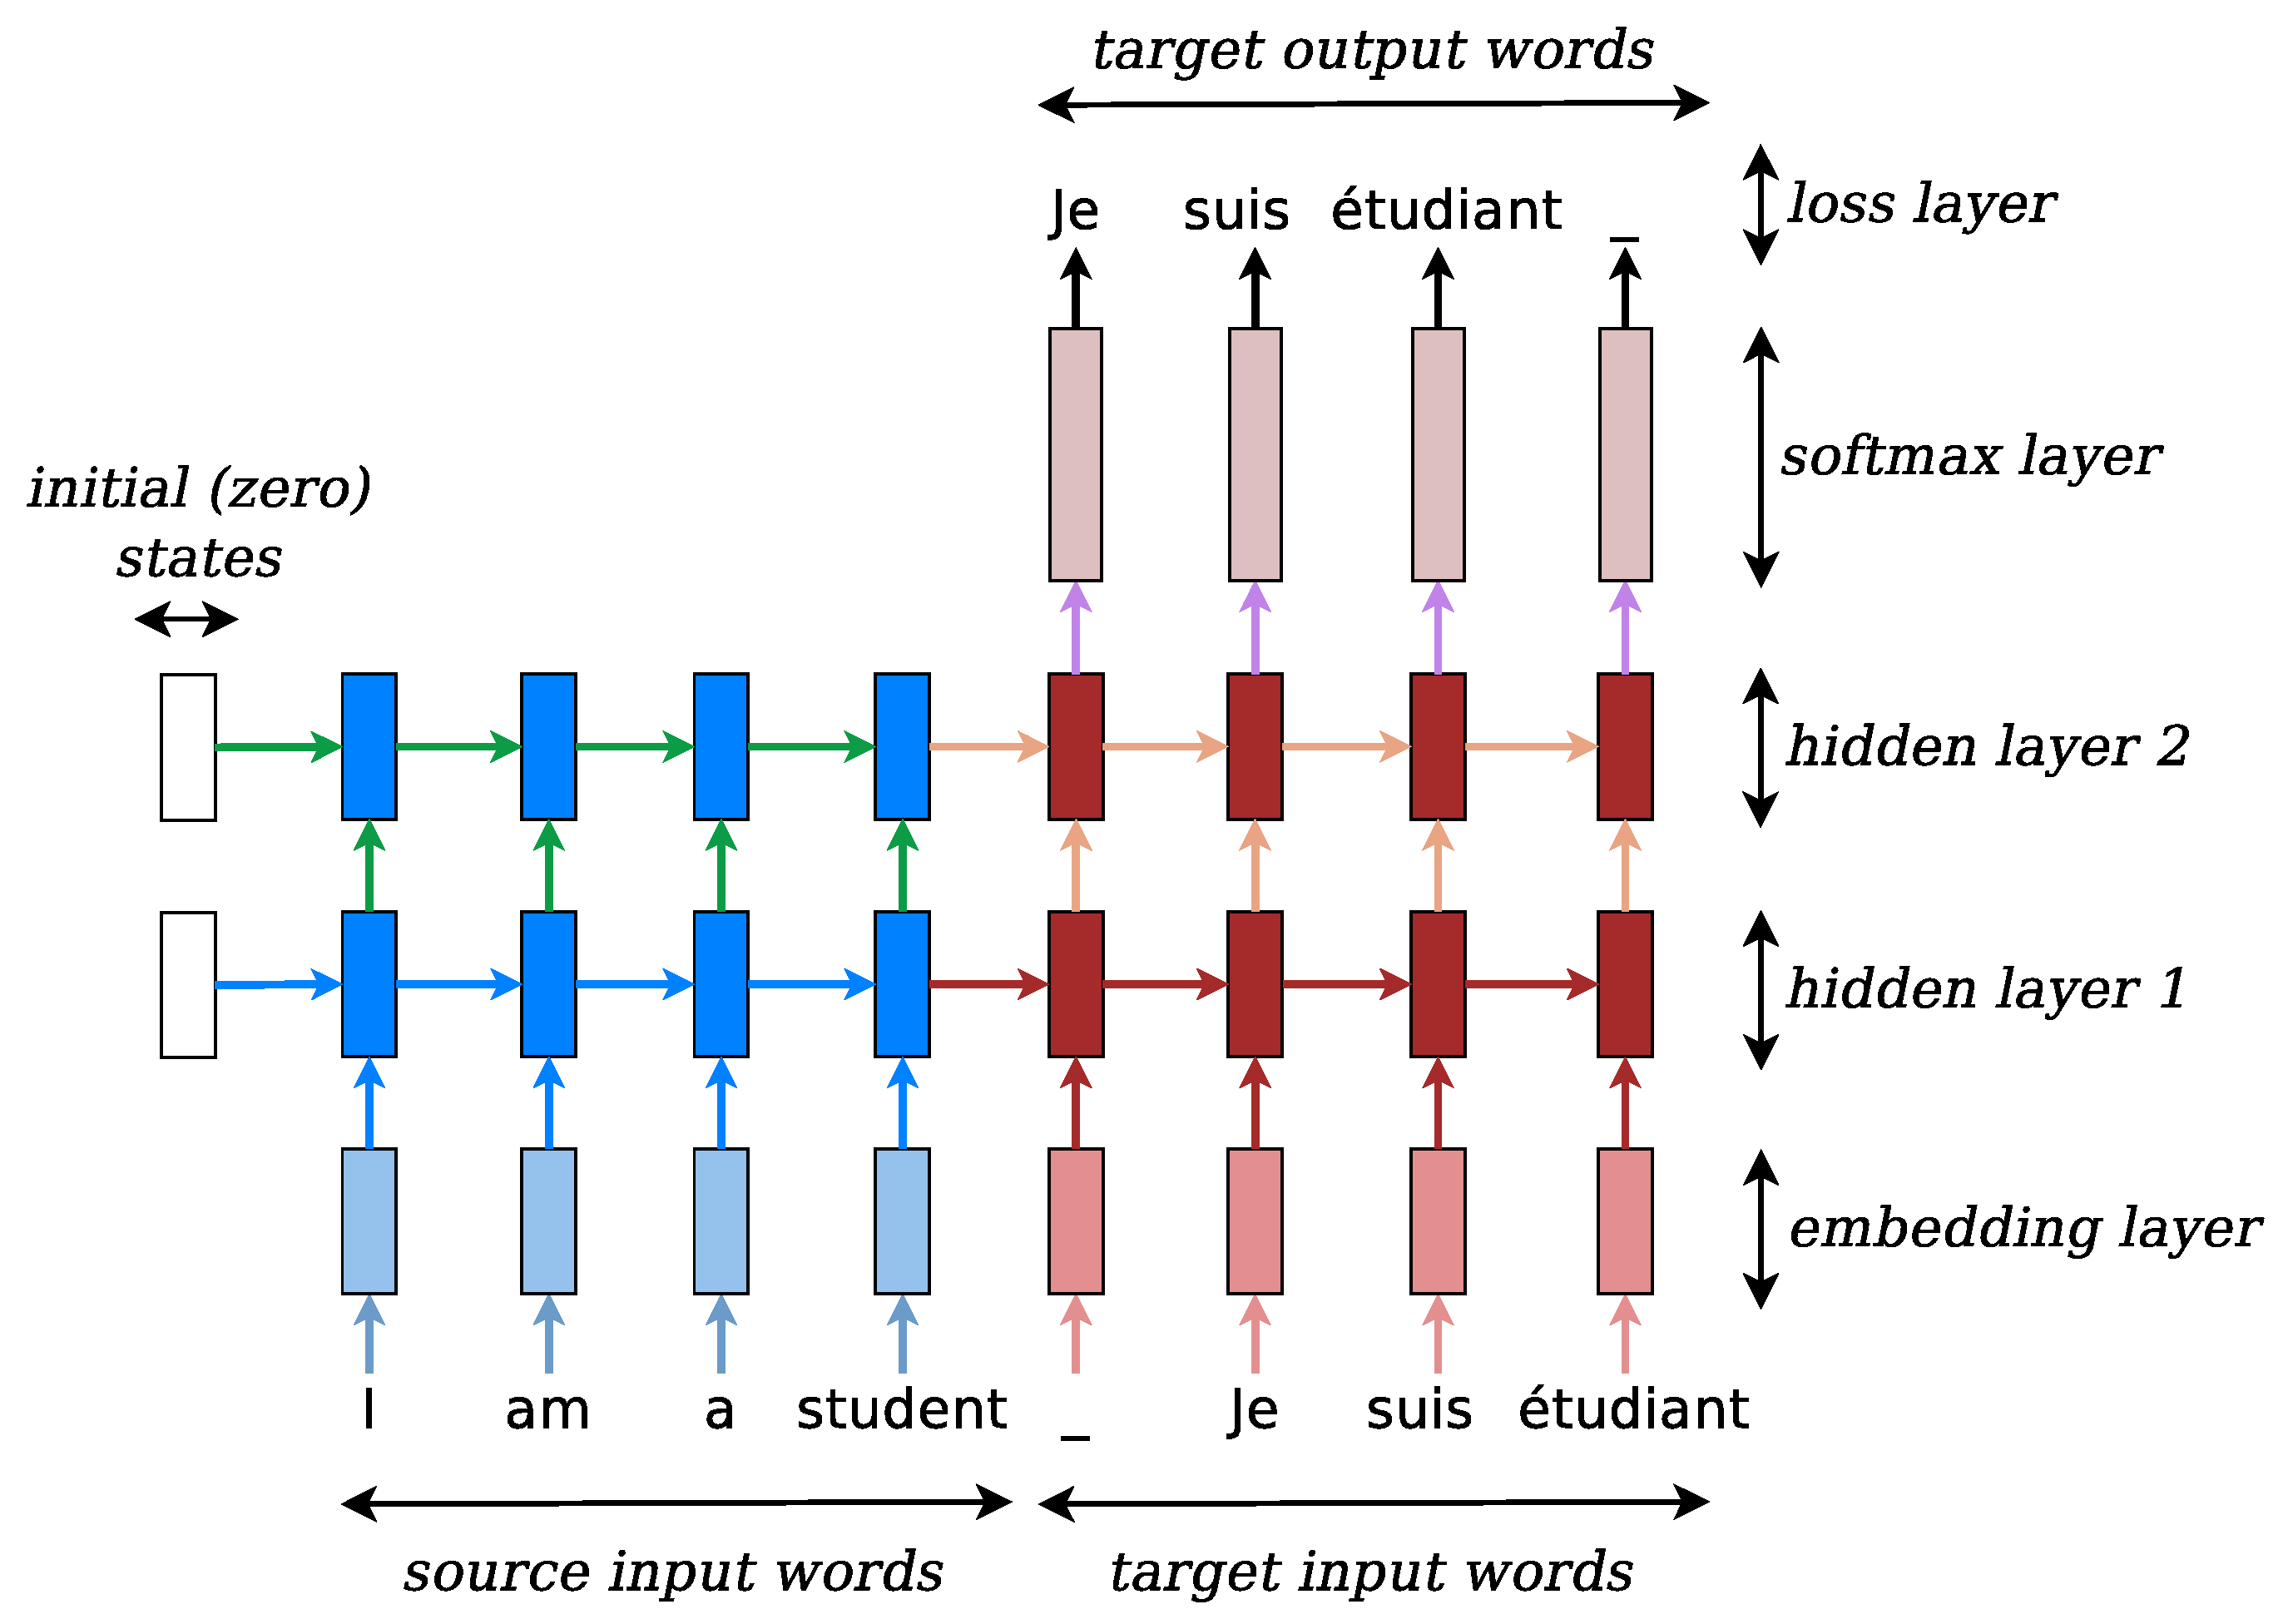
\includegraphics[width=1\textwidth, clip=true, trim= 0 0 0
0]{img/nmt_very_details.eps} % , angle=-90
\caption[Neural machine translation]{{\bf Neural machine translation} -- example of a deep recurrent
architecture proposed by \newcite{sutskever14} for
translating a source sentence \word{I am a student} into a target sentence
\word{Je suis \'{e}tudiant}. Here, \word{\texttt{\_}} marks the end of a sentence.
} 
\label{f:nmt_details}
\end{figure}

In this thesis, all my NMT models are deep multi-layer RNNs which are 
unidirectional and have an LSTM as the recurrent unit. I show an example of
such model in Figure~\ref{f:nmt_details}.
In this example, I train my model to translate a source sentence
\word{I am a student} into a target one \word{Je suis \'{e}tudiant}.
At a high level, my NMT models consist of two recurrent neural networks as
described in \secref{sec:rnn}: the {\it encoder} RNN simply consumes the input
source words without making any prediction; the {\it decoder}, on the other
hand, processes
the target sentence while predicting the next words. 

In more detail, at the bottom layer, the encoder and decoder RNNs receive as
{\it input} the following: first,
the source sentence, then a boundary marker \word{\_} which indicates the
transition from the encoding to the decoding mode, and the target sentence. 
Given these discrete words, the model looks up the source and target
embeddings to retrieve the corresponding word representations.
For this {\it embedding layer} to work, a vocabulary is chosen for each language, and
often the top $V$ frequent words are selected.
These embedding weights, one set per language, are learned during training.
While one can choose to initialize embedding weights with pretrained word
representations, such as word2vec \cite{mikolov13nips} and Glove
\cite{pennington2014}, I found, in this thesis, that these
embeddings can be initialized randomly and learned from scratch given large training datasets.

Once retrieved, the word embeddings are then fed as input into the main network, which consists
of two multi-layer RNNs `stuck together' --- an encoder for the source
language and a decoder for the target language. \edit{These two RNNs, in
principle, can share the same weights; however, in practice, I found that
having two different RNN parameters works better and less overfits to large
training datasets.}
The encoder RNN uses zero vectors as its starting states. The decoder, on the
other hand, needs to have access to the source information, so one simple way to
achieve that is to
initialize it with the last hidden state of the encoder.\footnote{This is not the only way to initialize the decoder,
e.g., \newcite{cho14} connect the last encoder state to every timestep in the
decoder as an extra input.} In Figure~\ref{f:nmt_details}, I pass  
the hidden state at the source word \word{student} to the decoder side.
The \emph{feed-forward} (vertical) weights connect
the hidden unit from the layer below to the upper one; whereas, the
\emph{recurrent} (horizontal) weights transfer the history knowlege from the previous
timestep to the next one.
Often, different weights can be used across the encoder and decoder as well as
across different layers; in the current example, I have 4 different LSTM
weight sets $\lstm$, detailed in \eq{e:lstm_notation}, over $\{\text{encoder,
decoder}\} \times \{1^{\text{st}}, 2^{\text{nd}} \text{ layer}\}$.
Finally, for each target word, the hidden state at the top layer is transformed by the
\emph{softmax} weights into a probability distribution over the target
vocabulary of size $V$ according to \eq{e:score} and \eq{e:prob}. 

\subsection{Training}
Training a neural machine translation system is similar to training a recurrent
language model that I have discussed in \secref{sec:rnn} except that we need to
handle the conditioning on source sentences.
The training objective for NMT is formulated as:
\begin{equation}
J = \sum_{(\src{},\tgt{}) \in \mathbb{D}} \nolimits -\log p(\tgt{}|\src{})
\label{e:j_t}
\end{equation}
Here, $\mathbb{D}$ refers to our parallel training corpus of source and target
sentence pairs $(x, y)$. Given the aforementioned NMT architecture,
computing the NMT loss for $(x, y)$ during the {\it forward} pass is
almost the same as how we compute the regular RNN loss on just $y$.
The only difference is that we have to first compute representations for the source
sentence $x$ to initialize the decoder RNN instead of just starting
from zero states. For the {\it backpropagation} phase, computing gradients for
the decoder is the same as what I have described in
Algorithm~\ref{a:lstm_bptt} for regular RNNs. The last hidden-state gradient
from the decoder is
passed back to the encoder. I then continue backpropagating through the encoder
in a similar fashion as that of the decoder but without any prediction losses.

More concretely, I present in
\algo{a:nmt_forward} details of the forward pass of an NMT model which uses
a deep multi-layer LSTM architecture. Since the encoder and decoder share
many operations in common, we combine the source sentence $x$ (length
$m_x$), the target sentence $y$ (length $m_y$), and the end-of-sentence markers
\word{\_} together to form an input sequence $s$ as shown in Line 1. We first start with the encoder weights and initial states
set to zero (lines~2-3). The algorithm switches to the decoder mode at time
$m_x + 1$ (line~5). The same LSTM codebase (lines~8-11) is used for both the
encoder and decoder in which embeddings are first looked up for the input
$s_t$; after that, hidden states as well as LSTM cell memories are built from the
bottom layer to the top one (the $L^{\text{th}}$ layer). 
In Line~10, \texttt{LSTM} refers
to the entire formulation in
Eq~\ref{e:lstm_detailed}-\ref{e:lstm_detailed_output}, which one can easily
replace with other hidden units such as RNN and GRU. Lastly, on the decoder
side, the top hidden state is used to predict the next symbol $s_{t+1}$
(line~13); then, a loss value $l_t$ and a probability distribution
$\prob{t}$ computed according to Eq~\ref{e:score}-\ref{e:prob} are returned.

\begin{algorithm}
\KwIn{source sentence $x$ of length $m_x$, target sentence $y$ of length $m_y$.}
\Parameter{encoder $\W{e}^{\text{encoder}}$, $\lstm^{\text{encoder}}$; 
decoder $\W{e}^{\text{decoder}}$, $\lstm^{\text{decoder}}$.}
\KwOut{loss $\MB{l}$ and other intermediate variables for backpropagation.} 

$s \leftarrow [x, \text{\_}, y, \text{\_}]$ \tcp*{Length of $s$ is $m_x + 1 +
m_y + 1$}
$\W{e}, \lstm^{(1..L)} \leftarrow \W{e}^{\text{encoder}},
\lstm^{\text{encoder}}$ \tcp*{Encoder weights}
$\hid{0}^{(1..L)}, \mem{0}^{(1..L)} \leftarrow \bm{0}$ \tcp*{Zero init} %^{(1..L)}, \bm{0}^{(1..L)}$ \tcp*{Starting states and memories}

\For{$t=1 \rightarrow (m_x + 1 + m_y)$}
{

\tcp{Decoder transition}
\If{$t == (m_x + 1)$}{
  $\W{e}, \lstm^{(1..L)} \leftarrow \W{e}^{\text{decoder}}, \lstm^{\text{decoder}}$ \; % \tcp{Decoder embeddings}
  %$\lstm^{(1..L)} \leftarrow \lstm^{\text{decoder}}$ \; % \tcp{Decoder multi-layer LSTMs}
}

\tcp{Multi-layer LSTM}
% x_t
$\hid{t}^{(0)} \leftarrow \text{\texttt{Emb\_LookUp}}(s_t, \W{e})$ \;
\For{$l=1 \rightarrow L$} {
  $\hid{t}^{(l)}, \mem{t}^{(l)} \leftarrow \text{\texttt{LSTM}}\paren{\hid{t-1}^{(l)},
  \mem{t-1}^{(l)}, \hid{t}^{(l-1)}, \lstm^{(l)}}$ \tcp*{LSTM hidden unit}
}

\tcp{Target-side prediction}
\If{$t \geq (m_x + 1)$}{
  $l_t, \prob{t} \leftarrow \text{\texttt{Predict}}(s_{t+1}, \hid{t}^{(L)},\W{hy})$ \;
}
}
\caption{NMT training algorithm -- {\it forward} pass.}
\label{a:nmt_forward}
\end{algorithm}


\begin{algorithm}
%$\W{e}, \lstm^{(1..L)} \leftarrow \W{e}^{\text{decoder}}, \lstm^{\text{decoder}}$ \tcp*{Decoder weights}
$d\hid{m_x + 1 + m_y}^{(1..L)}, d\mem{m_x + 1 + m_y}^{(1..L)} \leftarrow \bm{0}$ \tcp*{Cell and state gradients}
$d\lstm^{(1..L)}, d\W{e}, d\W{hy} \leftarrow \bm{0}$ \tcp*{Model weight gradients}

\For{$t=(m_x + 1 + m_y) \rightarrow 1$} {

\tcp{Encoder transition}
\If{$t == m_x$}{
  %$\W{e}, \lstm^{(1..L)} \leftarrow \W{e}^{\text{encoder}}, \lstm^{\text{encoder}}$ \tcp*{Encoder weights}
  $d\W{e}^{\text{decoder}}, d\lstm^{\text{decoder}} \leftarrow d\W{e},
  d\lstm^{(1..L)}$ \tcp*{Save decoder gradients}
  $d\lstm^{(1..L)}, d\W{e} \leftarrow \bm{0}$ \; %\tcp*{Zero init} %\;
}

\tcp{Target-side prediction}
\If{$t \geq (m_x + 1)$}{
  $d\hid{}, d\W{} \leftarrow
  \text{\texttt{Predict\_grad}}(s_{t+1}, \prob{t}, \hid{t}^{(L)})$\; %,\W{hy})$\;
  % \texttt{Accumulate}$(d\W{hy})$;
  $d\hid{t}^{(L)} \leftarrow d\hid{t}^{(L)} + d\hid{}$ \tcp*{\edit{Vertical  gradients}} %\;
  $d\W{hy} \leftarrow d\W{hy} + d\W{}$\;
}

\tcp{Multi-layer LSTM}
\For{$l=L \rightarrow 1$} {
  %\tcp{The first two returning gradients are for the previous timestep}
  \tcp{\edit{Recurrent  gradients}}
  $d\hid{t-1}^{(l)}, d\mem{t-1}^{(l)}, d\x{}, d\bm{T} \leftarrow 
  \text{\texttt{LSTM\_grad}}\paren{d\hid{t}^{(l)}, d\mem{t}^{(l)}, \hid{t-1}^{(l)},
  \mem{t-1}^{(l)}, \hid{t}^{(l-1)}}$ \;  %, \lstm^{(l)}
  % \texttt{Accumulate}$(d\lstm^{(l)})$;
  $d\hid{t}^{(l-1)} \leftarrow d\hid{t}^{(l-1)} + d\x{}$\tcp*{\edit{Vertical  gradients}}
  $d\lstm^{(l)} \leftarrow d\lstm^{(l)} + d\bm{T}$\;
}
$d\W{e} \leftarrow \text{\texttt{Emb\_grad\_update}}(s_t, d\hid{t}^{(0)}, d\W{e})$ \;

}
$d\W{e}^{\text{encoder}}, d\lstm^{\text{encoder}} \leftarrow d\W{e},
d\lstm^{(1..L)}$ \tcp*{Save encoder gradients}

\caption{NMT training algorithm -- {\it backpropagation} pass.}
\label{a:nmt_backward}
\end{algorithm}


%% BPTT
Next, I describe details of the backpropagation step in \algo{a:nmt_backward}.
A quick glance through the algorithm reveals many similarities compared to the
forward pass algorithm except that we have reversed the procedure. 
First, we initialize gradients of the recurrent layers at the final time step (line 1)
as well the model weights on the decoder size (line 2) to zero.
At time $m_x$, we switch to the encoder mode by saving the currently
accumulated LSTM and embedding gradients for the decoder (line 5) and 
starting to accumulate gradients for the encoder weights (line 6). 
%Individual gradients are computed in Line~13-23. 
Thanks to the backpropagation
procedure presented earlier for LSTM, we can simplify the core NMT gradient
computation (lines~8-18) by making the following two referents: (a)
\texttt{Predict\_grad} (lines~2-4 of \algo{a:lstm_bptt}) which computes gradients for the target-side
losses with respect to the hidden states at the top layer and the softmax
weights $\W{hy}$; and (b) \texttt{LSTM\_grad} (lines~5-15 of
\algo{a:lstm_bptt}) which computes gradients for inputs to LSTM and the LSTM
weights per layer $\lstm^{(l)}$. It is important to note that in Lines 10 and 15 of
\algo{a:nmt_backward}, we add the gradients (flowing vertically from either the
loss or the upper LSTM layer) to the gradient of the below layer (which already
contains the gradient backpropagated horizontally)
instead of overriding it. In Line 18, we perform
sparse updates on the corresponding embedding matrix for participating words
only. Lastly, implementation wise, one can save memory by using a single copy of
$d\hid{}^{(1..L)}$ and $d\mem{}^{(1..L)}$ for all time steps and overwriting the values
whenever we transition from timesteps $t$ to $t-1$ (line 14).
% mention bucketing and batching

\subsection{Testing}
Having trained an NMT model, we, of course, need to be able to use it to
translate, or decode, unseen source sentences! This section explains a few different ways to 
accomplish this goal and how to decode with an ensemble of models.

%\paragraph{Greedy Decoder} 
The simplest strategy to translate a source sentence is to perform {\it greedy
decoding} which I illustrate in \figref{f:nmt_test}. The idea is simple: (a) we
first encode the source sentence,
\word{I am a student} in our example, similar to the training process; (b) the
decoding process is started as soon as
an end-of-sentence marker \word{\_} for the source sentence is fed as an input; and (c) for each
timestep on the decoder side,
we pick the most likely word (a greedy choice), e.g., \word{moi} has the highest
translation probability in the first
decoding step, then use it as an input to the next timestep, and continue
until the end-of-sentence marker \word{\_} is produced as an output symbol. Step
(c) is what makes testing different from training: unlike training in which
correct target words in $y$ are always fed as an input, testing, on the other
hand, uses words predicted by the model.

\begin{figure}[tbh!]
\centering
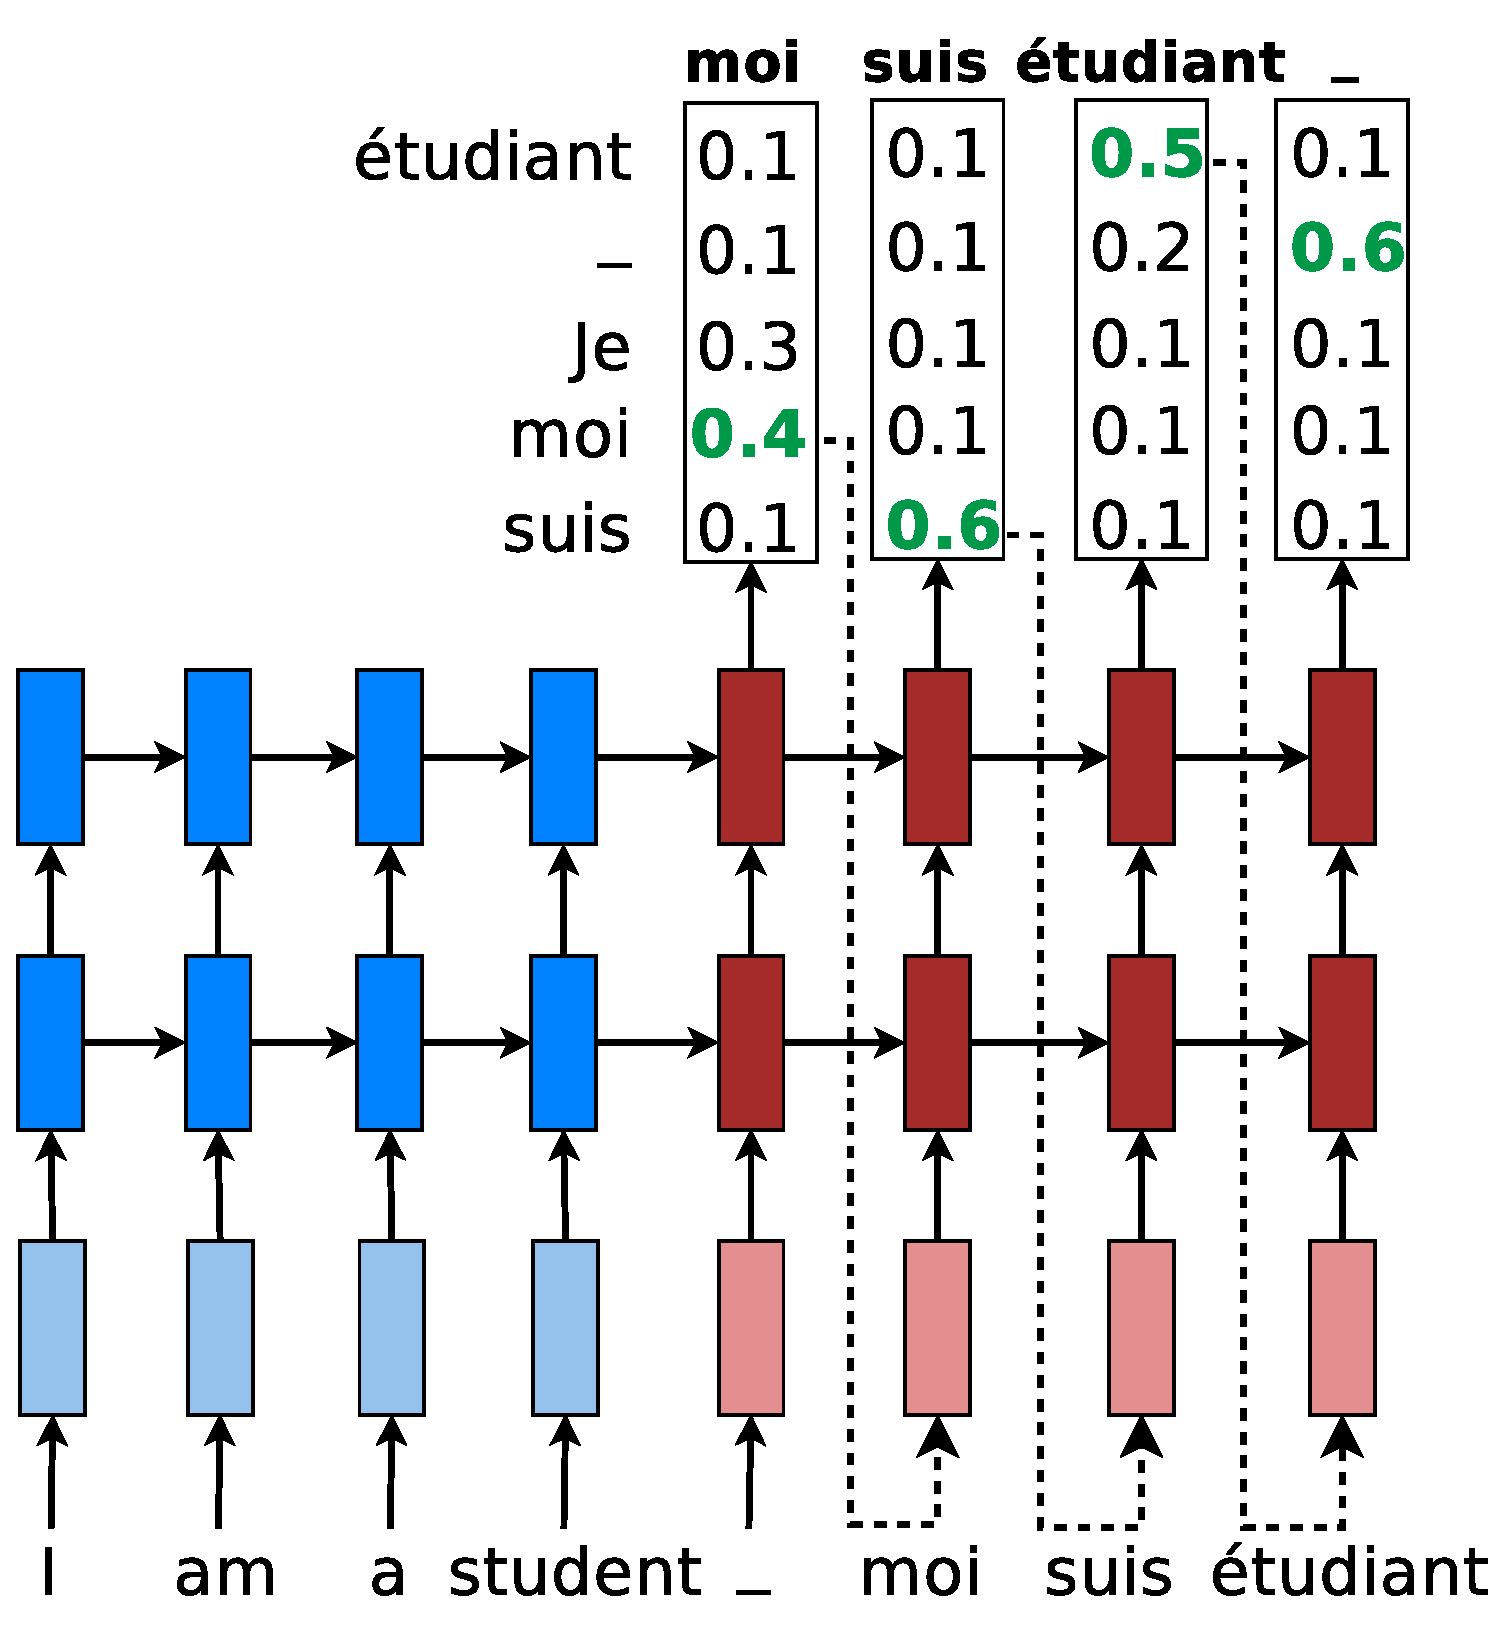
\includegraphics[width=0.6\textwidth, clip=true, trim= 0 0 0
0]{img/nmt_test.eps} % , angle=-90
\caption[Greedy Decoding]{{\bf Greedy Decoding}
-- example of how a trained NMT model produces a translation for a
source sentence \word{I am a student} using greedy search.
} 
\label{f:nmt_test}
\end{figure}

More concretely, I adopt the NMT forward algorithm to arrive at the greedy
decoding strategy in \algo{a:nmt_greedy}. I present the greedy
algorithm in a slightly more abstract way by reusing elements of the NMT forward
pass in \algo{a:nmt_forward}. First, we run through the encoder in Line 1 to obtain a
representation $\hid{0}, \mem{0}$ for the source sentence $x$ (length $m_x$). We
then use the end-of-sentence marker \word{\_} as an input to start the decoding
process and restrict the final translation to have a maximum length of
$\alpha*m_x$.\footnote{We often set $\alpha$ to $1.5$. } At each timestep on the
decoder side, we call \texttt{MultiLayerLSTM}, which refers to Lines~8-11 in
\algo{a:nmt_forward}, to build up representations over $L$ stacking LSTM layers. The hidden
state at the top layer is used to compute the predictive distribution $\prob{t}$
from which we make a greedy choice to produce the index of the translation word
at that timestep (line~7). The process ends when we have produced the marker
\word{\_} as a translation word or when the translation length exceeds the
length threshold.

\begin{algorithm}
$\hid{0}, \mem{0} \leftarrow \text{Encoder}(x, \W{e}^{\text{encoder}}, \lstm^{\text{encoder}})$ \;
$t \leftarrow 1$ \;
$y_1 \leftarrow \_$ \;
\While(\tcp*[f]{Length factor $\alpha \geq 1$}){$t \leq \alpha * m_x$} {
  $\hid{t}, \mem{t} \leftarrow \text{\texttt{MultiLayerLSTM}}\paren{\hid{t-1},
  \mem{t-1}, y_t, \W{e}^{\text{decoder}}, \lstm^{\text{decoder}}}$ \;

  $\prob{t} \leftarrow \text{\texttt{Softmax}}(\hid{t}^{(L)},\W{hy})$ \;
  $y_{t+1} \leftarrow \argmax_i \prob{t}(i)$ \tcp*{\bfit{Greedy} choice}
  \If(\tcp*[f]{Ending condition}){$y_{t+1} == \Index(\_)$} {
    break\;
  }

  $t \leftarrow t+1$
}
\Return $y_{2..t}$

\caption{NMT {\it greedy} decoding algorithm.}
\label{a:nmt_greedy}
\end{algorithm}

%\paragraph{Beam-search Decoder} 

For NMT, it turns out that such a simple strategy of greedy decoding can produce
very good translations \cite{sutskever14}. However, to achieve a better result,
a more popular strategy is to use a {\it beam-search} decoding algorithm which has been the
core of phrase-based statistical machine translation for years \cite{Koehn:2003:SMT}.
Unlike phrase-based SMT, NMT has a much simpler beam-search decoding algorithm
since it generates translations word-by-word from left to right \edit{and does 
not have to explicitly explore different places on the source side to pay
attention to}.\footnote{\edit{In SMT, a source coverage set is maintained to
indicate which words have been translated. As translation progresses, an SMT 
system base on the coverage set and pick untranslated source words to continue.
Such an idea of coverage set later re-emerges in NMT which I will describe more in Chapter~\ref{c:conclude}.}}
One can modify
the greedy decoding algorithm as follows to build a beam-search decoder: (a) at
each timestep on the decoder side, we keep track of the top $B$ (the beam size) best
translations together with their corresponding hidden states; (b) in Line 7 of
\algo{a:nmt_greedy}, instead of applying argmax, we select the top $B$ most
likely words; and (c) given $B$ previous best translation $\times B$ best words, we
select a new set of $B$ best translations for the current timestep based on the
combined scores (previous translation scores + current word translation scores).
Extra care needs to be taken to make sure that in step (c) we select correct
hidden states for the new set of $B$ best translations. \newcite{sutskever14}
observed that for NMT, a minimal beam size of $2$ already provides a significant
boost in translation quality. A beam of size $10$ is often used, which is
significant smaller that what phrase-based SMT tends to use, about $100-200$.

Furthermore, to achieve the very best result, one simple strategy which has been
widely adopted for deep neural networks is to use an ensemble of models. For NMT
decoding, using multiple models is pretty straightforward. The idea is that each
model produces a distribution at each timestep in the decoder (line~6 of
\algo{a:nmt_greedy}). These different distributions are then averaged to produce
a new ensemble distribution which we can use for both greedy and beam-search
decoders as if we decode from a single model.

\edit{In summary, I have covered all the necessary background knowledge to understand
this thesis entirely. We start with language modeling, an important concept in
natural language processing, which turns out to be the basis of NMT. One can
simply view NMT as a source-conditioned language model. To understand how NMT systems work, I
have covered the fundamentals of recurrent neural networks which allow us to
handle variable-length sequences, in our case, the sentences. We have particularly 
studied Long Short-term Memory, a specific type of RNN that
is more effective at handling long sequences, in depth. Finally, given these building blocks,
language modeling and RNN, I have discussed NMT in detail from training to testing.}
